% !TEX TS-program = pdflatex
% !TEX encoding = UTF-8 Unicode

% This is a simple template for a LaTeX document using the "article" class.
% See "book", "report", "letter" for other types of document.

\documentclass[11pt]{scrartcl} % use larger type; default would be 10pt

\usepackage[utf8]{inputenc} % set input encoding (not needed with XeLaTeX)

%%% Examples of Article customizations
% These packages are optional, depending whether you want the features they provide.
% See the LaTeX Companion or other references for full information.

%%% PAGE DIMENSIONS
\usepackage{geometry} % to change the page dimensions
\geometry{a4paper} % or letterpaper (US) or a5paper or....
% \geometry{margin=2in} % for example, change the margins to 2 inches all round
% \geometry{landscape} % set up the page for landscape
%   read geometry.pdf for detailed page layout information

\usepackage{graphicx} % support the \includegraphics command and options

% \usepackage[parfill]{parskip} % Activate to begin paragraphs with an empty line rather than an indent

%%% PACKAGES
\usepackage{booktabs} % for much better looking tables
\usepackage{array} % for better arrays (eg matrices) in maths
\usepackage{paralist} % very flexible & customisable lists (eg. enumerate/itemize, etc.)
\usepackage{verbatim} % adds environment for commenting out blocks of text & for better verbatim
\usepackage{subfig} % make it possible to include more than one captioned figure/table in a single float
\usepackage{graphicx}
% These packages are all incorporated in the memoir class to one degree or another...
\usepackage{hyperref}

%%% SECTION TITLE APPEARANCE
\usepackage{sectsty}
\allsectionsfont{\sffamily\mdseries\upshape} % (See the fntguide.pdf for font help)
% (This matches ConTeXt defaults)

%%% ToC (table of contents) APPEARANCE
\usepackage[nottoc,notlof,notlot]{tocbibind} % Put the bibliography in the ToC
\usepackage[titles,subfigure]{tocloft} % Alter the style of the Table of Contents
\renewcommand{\cftsecfont}{\rmfamily\mdseries\upshape}
\renewcommand{\cftsecpagefont}{\rmfamily\mdseries\upshape} % No bold!


\usepackage{amssymb}
\usepackage{amsmath}
\usepackage{mathcomp}
%\usepackage{colortbl}
\usepackage{dsfont}
\usepackage{amsfonts}
\usepackage{cancel}

%%% KV-Diagramme
%\usepackage[ngerman]{babel}
\input kvmacros

%%% Graphen
\usepackage{tikz}
\usetikzlibrary{intersections}
\usetikzlibrary{calc}

% last page
\usepackage{pageslts}

%%% END Article customizations

%%% HEADERS & FOOTERS
\usepackage{fancyhdr} % This should be set AFTER setting up the page geometry
%\usepackage{scrpage2} % Another package (only use fancyhdr or scrpage2)
\pagestyle{fancy} % options: empty , plain , fancy
\renewcommand{\headrulewidth}{1.2pt} % customise the layout...
\renewcommand{\footrulewidth}{0.1pt} % customise the layout...
\lhead{MACHINE LEARNING 1\\Andres Fernandez -- 5692442 -- fr\_andres@msn.com}\chead{}\rhead{Exercise Sheet 7 \\December 19
  , 2016}
\lfoot{}\cfoot{\thepage/\lastpageref{LastPages}}\rfoot{}



%%% THE SYMBOLS FOR ``DEPENDENT'' AND ``INDEPENDENT''
\newcommand{\CI}{\mathrel{\text{\scalebox{1.07}{$\perp\mkern-10mu\perp$}}}} % independent
\newcommand{\nCI}{\cancel{\mathrel{\text{\scalebox{1.07}{$\perp\mkern-10mu\perp$}}}}} % dep
%% THE SYMBOL FOR DOESN'T IMPLY
\newcommand{\notimplies}{%
  \mathrel{{\ooalign{\hidewidth$\not\phantom{=}$\hidewidth\cr$\implies$}}}}

%%% The "real" document content comes below...


\begin{document}


         \vspace{5mm}
\section*{Exercise 3}
Please see the  Python2 script {\it fernandez\_blatt7.py} attached to this PDF for the details on how this figures were generated.

           \begin{figure}[ht]
	   \centering
           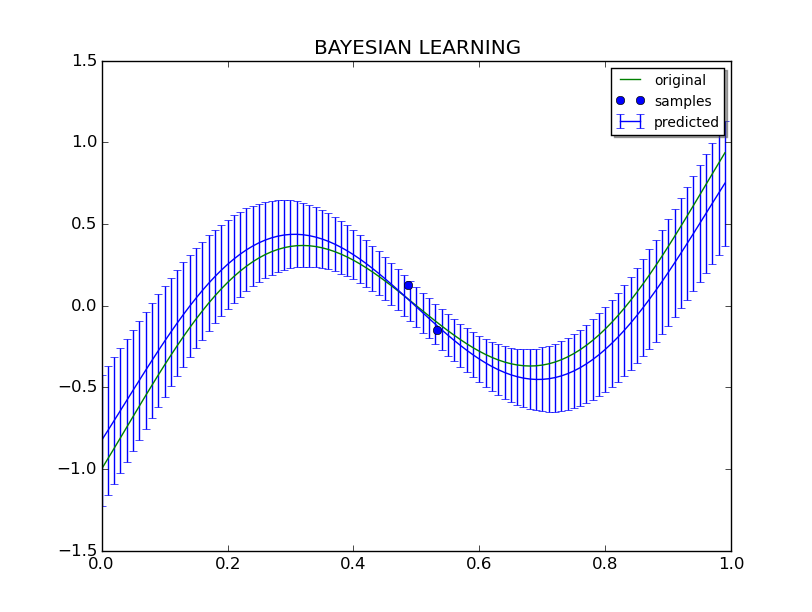
\includegraphics[width=0.7\textwidth, angle=0]{2samples.png}
	   \caption{With only two points generated, the posterior isn't able to overcome the noise}
	   \label{fig2}
           \end{figure}
           \begin{figure}[ht]
	   \centering
           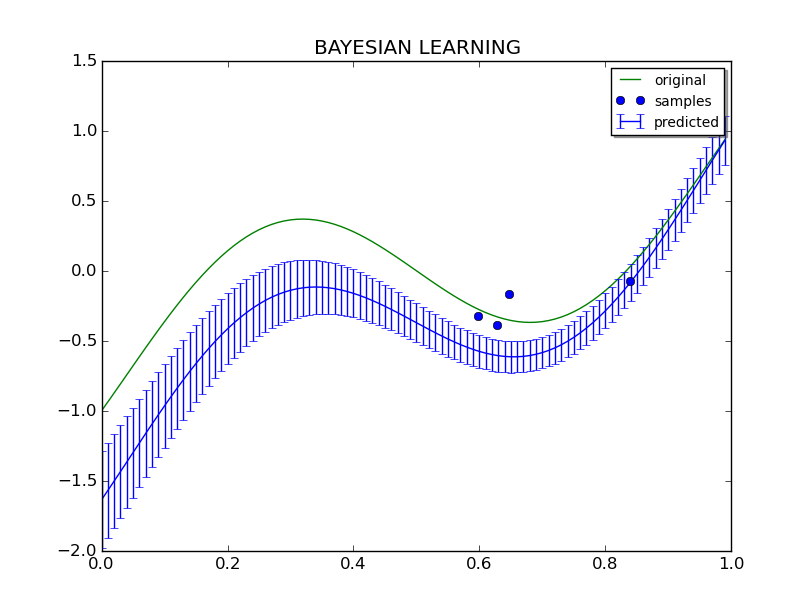
\includegraphics[width=0.7\textwidth, angle=0]{4samples.png}
	   \caption{With only two points generated, the prior distribution has predominance. The likelihood provides a linear function space because we have three dimensions, and 2 points, and both of them are multiplied resulting in the observed intersection}
	   \label{fig2}
           \end{figure}
           \begin{figure}[ht]
	   \centering
           \includegraphics[width=0.7\textwidth, angle=0]{.png}
	   \caption{The bayesian estimation progresses greatly in the first steps. This is very useful in small datasets}
	   \label{fig2}
           \end{figure}
           \begin{figure}[ht]
	   \centering
           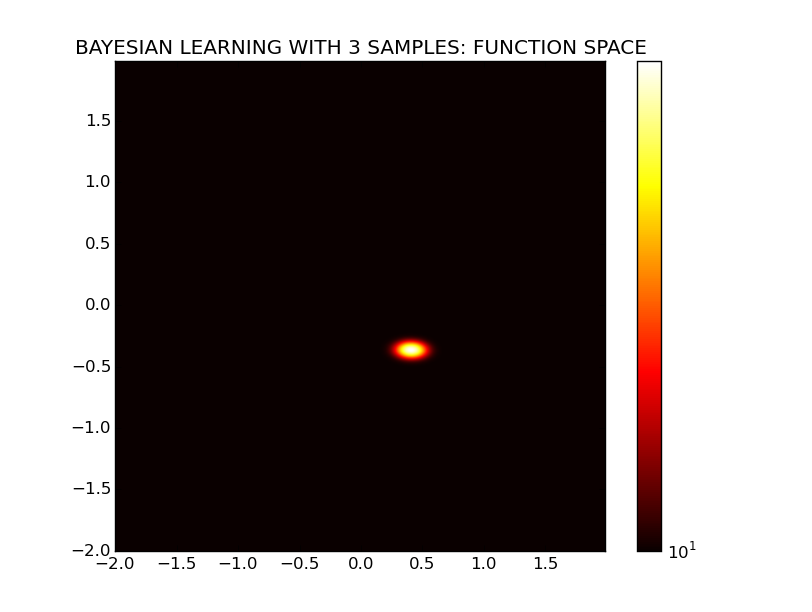
\includegraphics[width=0.7\textwidth, angle=0]{f3.png}
	   \caption{With 3 points it is already possible to limit all dimensions. This plot is the multiplication between the plot before, and the estimation provided by the new point, as it can be seen above in the definition of the likelihood}

	   \label{fig2}
           \end{figure}
           \label{fig2}
           \end{figure}
           \label{fig2}
           \end{figure}
           \begin{figure}[ht]
	   \centering
           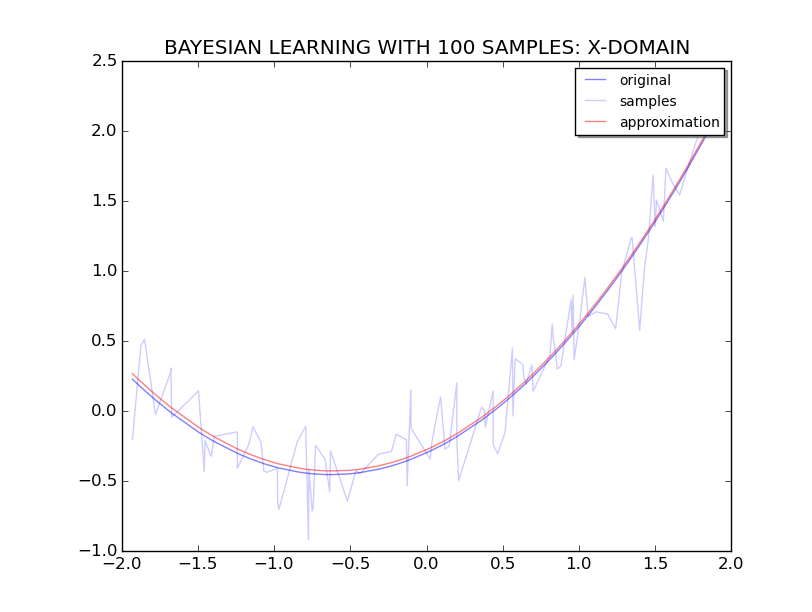
\includegraphics[width=0.7\textwidth, angle=0]{x100.png}
	   \caption{with 100 samples, the approximation is already very percise}
	   \label{fig2}
           \end{figure}
           \begin{figure}[ht]
	   \centering
           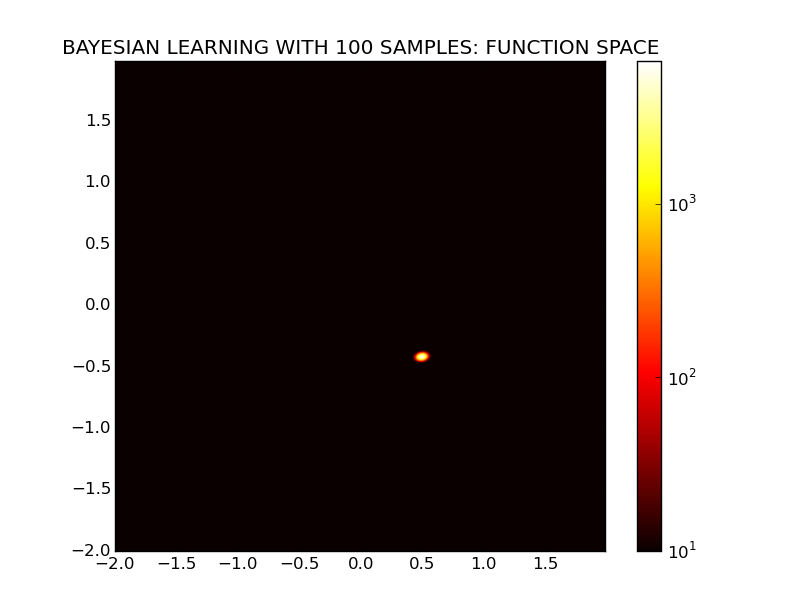
\includegraphics[width=0.7\textwidth, angle=0]{f100.png}
	   \caption{and the feasible function space is extremely reduced, but never to a singular point: the main advantage of bayesian learning is that each possible outcome can be analyzed, and not only the maxima like in the classical ML algorithms. This enable a more explicit formulation of the assumptions and biases, which may help to explain better the existing models}
	   \label{fig2}
           \end{figure}


           

\end{document}




\begin{flushright}
  $\square$\\
\end{flushright}
